%%%
%
% $Autor: Müller, Hinrichs $
% $Datum: 2026-06-09 14:18:35Z $
% $Pfad: UltraschallradarAutomatisierungstechnik/report/Contents/General/Processing.tex $
% $Version: 1 $
%
% Project: 
%
%%%


\chapter{Processing 4.3}\label{chap:Processing_IDE_Installation}
Dieses Kapitel liefert eine detaillierte Einführung in die Entwicklungsumgebung Processing, einschlei\ss lich ihrer zentralen Funktionen, grafischen Fähigkeiten und der grundlegenden Arbeitsweise. Es erläutert die einzelnen Bestandteile der Entwicklungsumgebung, beschreibt den Installationsprozess anhand klar strukturierter Schritte für verschiedene Plattformen und bietet eine Anleitung zur Konfiguration der Programmierumgebung für die serielle Datenverarbeitung.

\section{Processing Beschreibung}
\label{chap:Processing_Beschreibung}
Processing ist eine flexible, quelloffene (Open-Source) Entwicklungsumgebung und eine objektorientierte Programmiersprache, die ursprünglich im Jahr 2001 am MIT Media Lab initiiert wurde. Sie wurde gezielt entwickelt, um Designern, Künstlern und Ingenieuren den Einstieg in die Programmierung visueller, interaktiver Anwendungen und Grafiken zu erleichtern. Basiert auf der Java-Plattform, bietet Processing eine stark vereinfachte Syntax, die komplexe Grafikoperationen wie das Zeichnen von Primitiven, das Verarbeiten von Transformationsmatrizen und das Rendern in Echtzeit mit nur wenigen Zeilen Code ermöglicht. Als plattformübergreifende Anwendung läuft die integrierte Entwicklungsumgebung (IDE) nativ unter Windows, Linux und macOS \cite{Reas:2014}.
\\
In Analogie zur Arduino-Umgebung werden Programme in Processing ebenfalls als „Sketche“ bezeichnet. Diese Skripte definieren die Geometrie, Farbwerte und das Verhalten des Anzeigefensters, das sich bei der Ausführung des Codes öffnet. Ein Processing-Sketch wird standardmä\ss ig mit der Dateiendung \menu{.pde} abgespeichert. Nach dem Starten des Programms übersetzt die IDE den Quellcode intern in Java-Bytecode, bindet die erforderlichen Grafikbibliotheken ein und führt die Applikation als eigenständiges Java-Applet innerhalb eines dedizierten Display-Fensters aus. Dies erlaubt eine unmittelbare visuelle Rückmeldung über das programmierte Verhalten, was insbesondere bei der Echtzeit-Visualisierung von Sensordaten von gro\ss em Vorteil ist \cite{Reas:2014}.
\\
Die integrierte Entwicklungsumgebung von Processing setzt sich im Wesentlichen aus drei funktionalen Ebenen zusammen: dem Code-Editor mit der darüberliegenden Toolbar, dem Nachrichtenbereich für den Systemstatus und der Konsole im unteren Abschnitt. Während der Editor das Schreiben des Quellcodes inklusive Syntax-Hervorhebung übernimmt, dient die Konsole der Ausgabe von Fehlermeldungen (Compiler-Errors) sowie textbasierten Debug-Informationen, die mittels spezifischer Ausgabebefehle generiert werden \cite{Reas:2014}.
\\
In der aktuellen Version von Processing kommt der Toolbar am oberen Rand des Editor-Fensters eine zentrale Bedeutung zu. Sie ist im Vergleich zu IDEs minimalistisch gehalten, um den Fokus auf den kreativen und funktionalen Code zu lenken. Über das Menü „Skript“ oder direkt über die Symbole der Toolbar lassen sich Programme ausführen, stoppen oder für die plattformunabhängige Weitergabe als eigenständige Applikation exportieren. Über den Menüpunkt „Beispiele“ bietet Processing zudem eine umfangreiche Sammlung vorgefertigter Skripte aus den Bereichen Grafik, Interaktion, Mathematik und Netzwerkkonstruktion, die als fundierte Grundlage für eigene Entwicklungen herangezogen werden können \cite{Reas:2014}.
\newpage
Die zentrale Benutzeroberfläche zum schreiben des Codes sieht wie folgt aus:
\begin{center}
	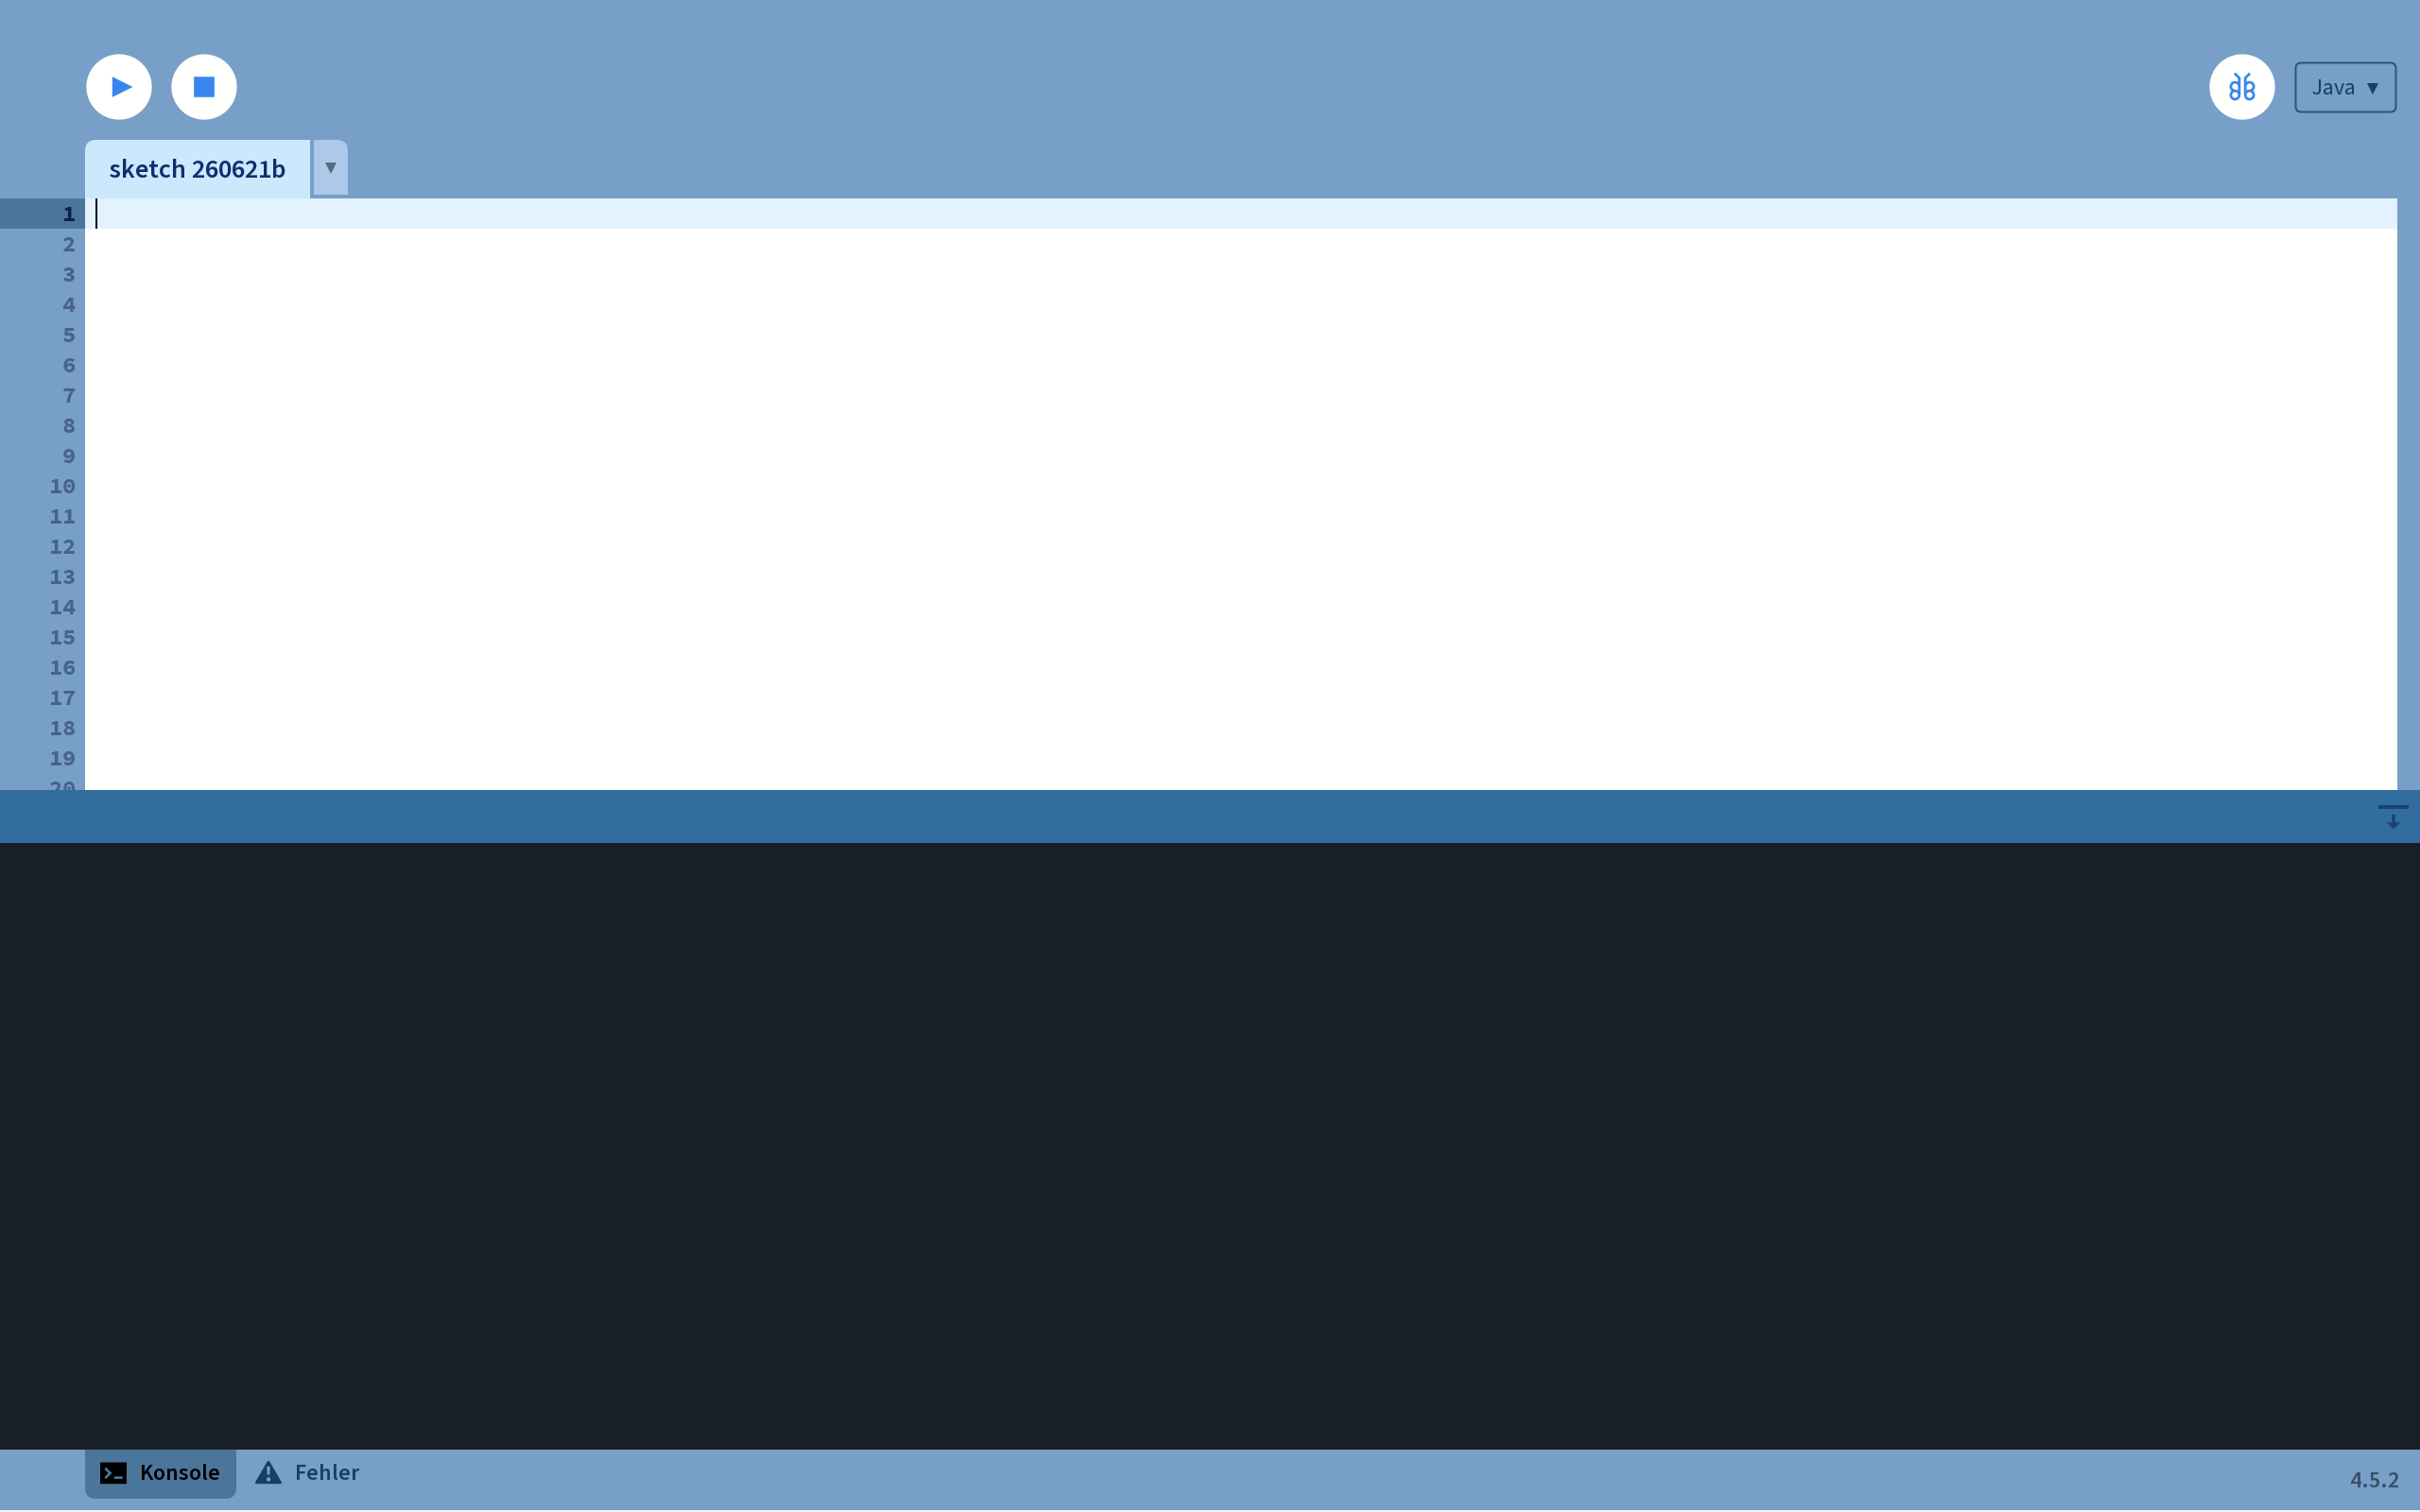
\includegraphics[width=\linewidth]{../Images/Processing/menuboard_processing}
\end{center}
\bigskip

\begin{itemize}
	\item[\hbox{
\includegraphics[viewport=0 0 40 40, clip=true, height=12pt]{../Images/Processing/MenuButton_Run}}]
	Das Wiedergabe-Symbol (Play) wird verwendet, um den geschriebenen Code zu \menu{Ausführen}. Die IDE kompiliert das Programm, öffnet das grafische Ausgabefenster und startet die Anwendung.
	\item[\hbox{
\includegraphics[viewport=0 0 40 40, clip=true, height=12pt]{../Images/Processing/MenuButton_Stop}}] 
	Das Quadrat-Symbol \menu{Stoppen} beendet die Ausführung des aktuell laufenden Sketches sofort und schlie\ss t das dazugehörige grafische Ausgabefenster. 
\end{itemize}

\section{Installation von Processing}
\label{chap:Installation_von_Processing}

\subsection{Download von Processing}
Die Erstellung von grafischen Oberflächen zur Datenvisualisierung erfolgt über die Processing-Entwicklungsumgebung, die sich als mächtiges Werkzeug für die Verknüpfung von Hardware-Rohdaten mit visuellen Elementen etabliert hat. Processing steht als Open-Source-Software kostenlos zur Verfügung und erfordert für die reine Ausführung innerhalb der IDE keine komplexe lokale Vorinstallation von Java-Entwicklungsumgebungen, da eine passende Java-Laufzeitumgebung (JRE) direkt in den Softwarepaketen integriert ist \cite{P}.

Die Distributionen sind für alle gängigen Desktop-Betriebssysteme verfügbar. Der Zugriff auf die offiziell verifizierten Softwarepakete erfolgt über die Webpräsenz der Entwicklergemeinschaft unter \HREF{https://processing.org/download/}{Processing-Software}. Ein Überblick über das Download-Verzeichnis ist in Abbildung~\ref{fig:Download_Processing} dargestellt.
\begin{center}
	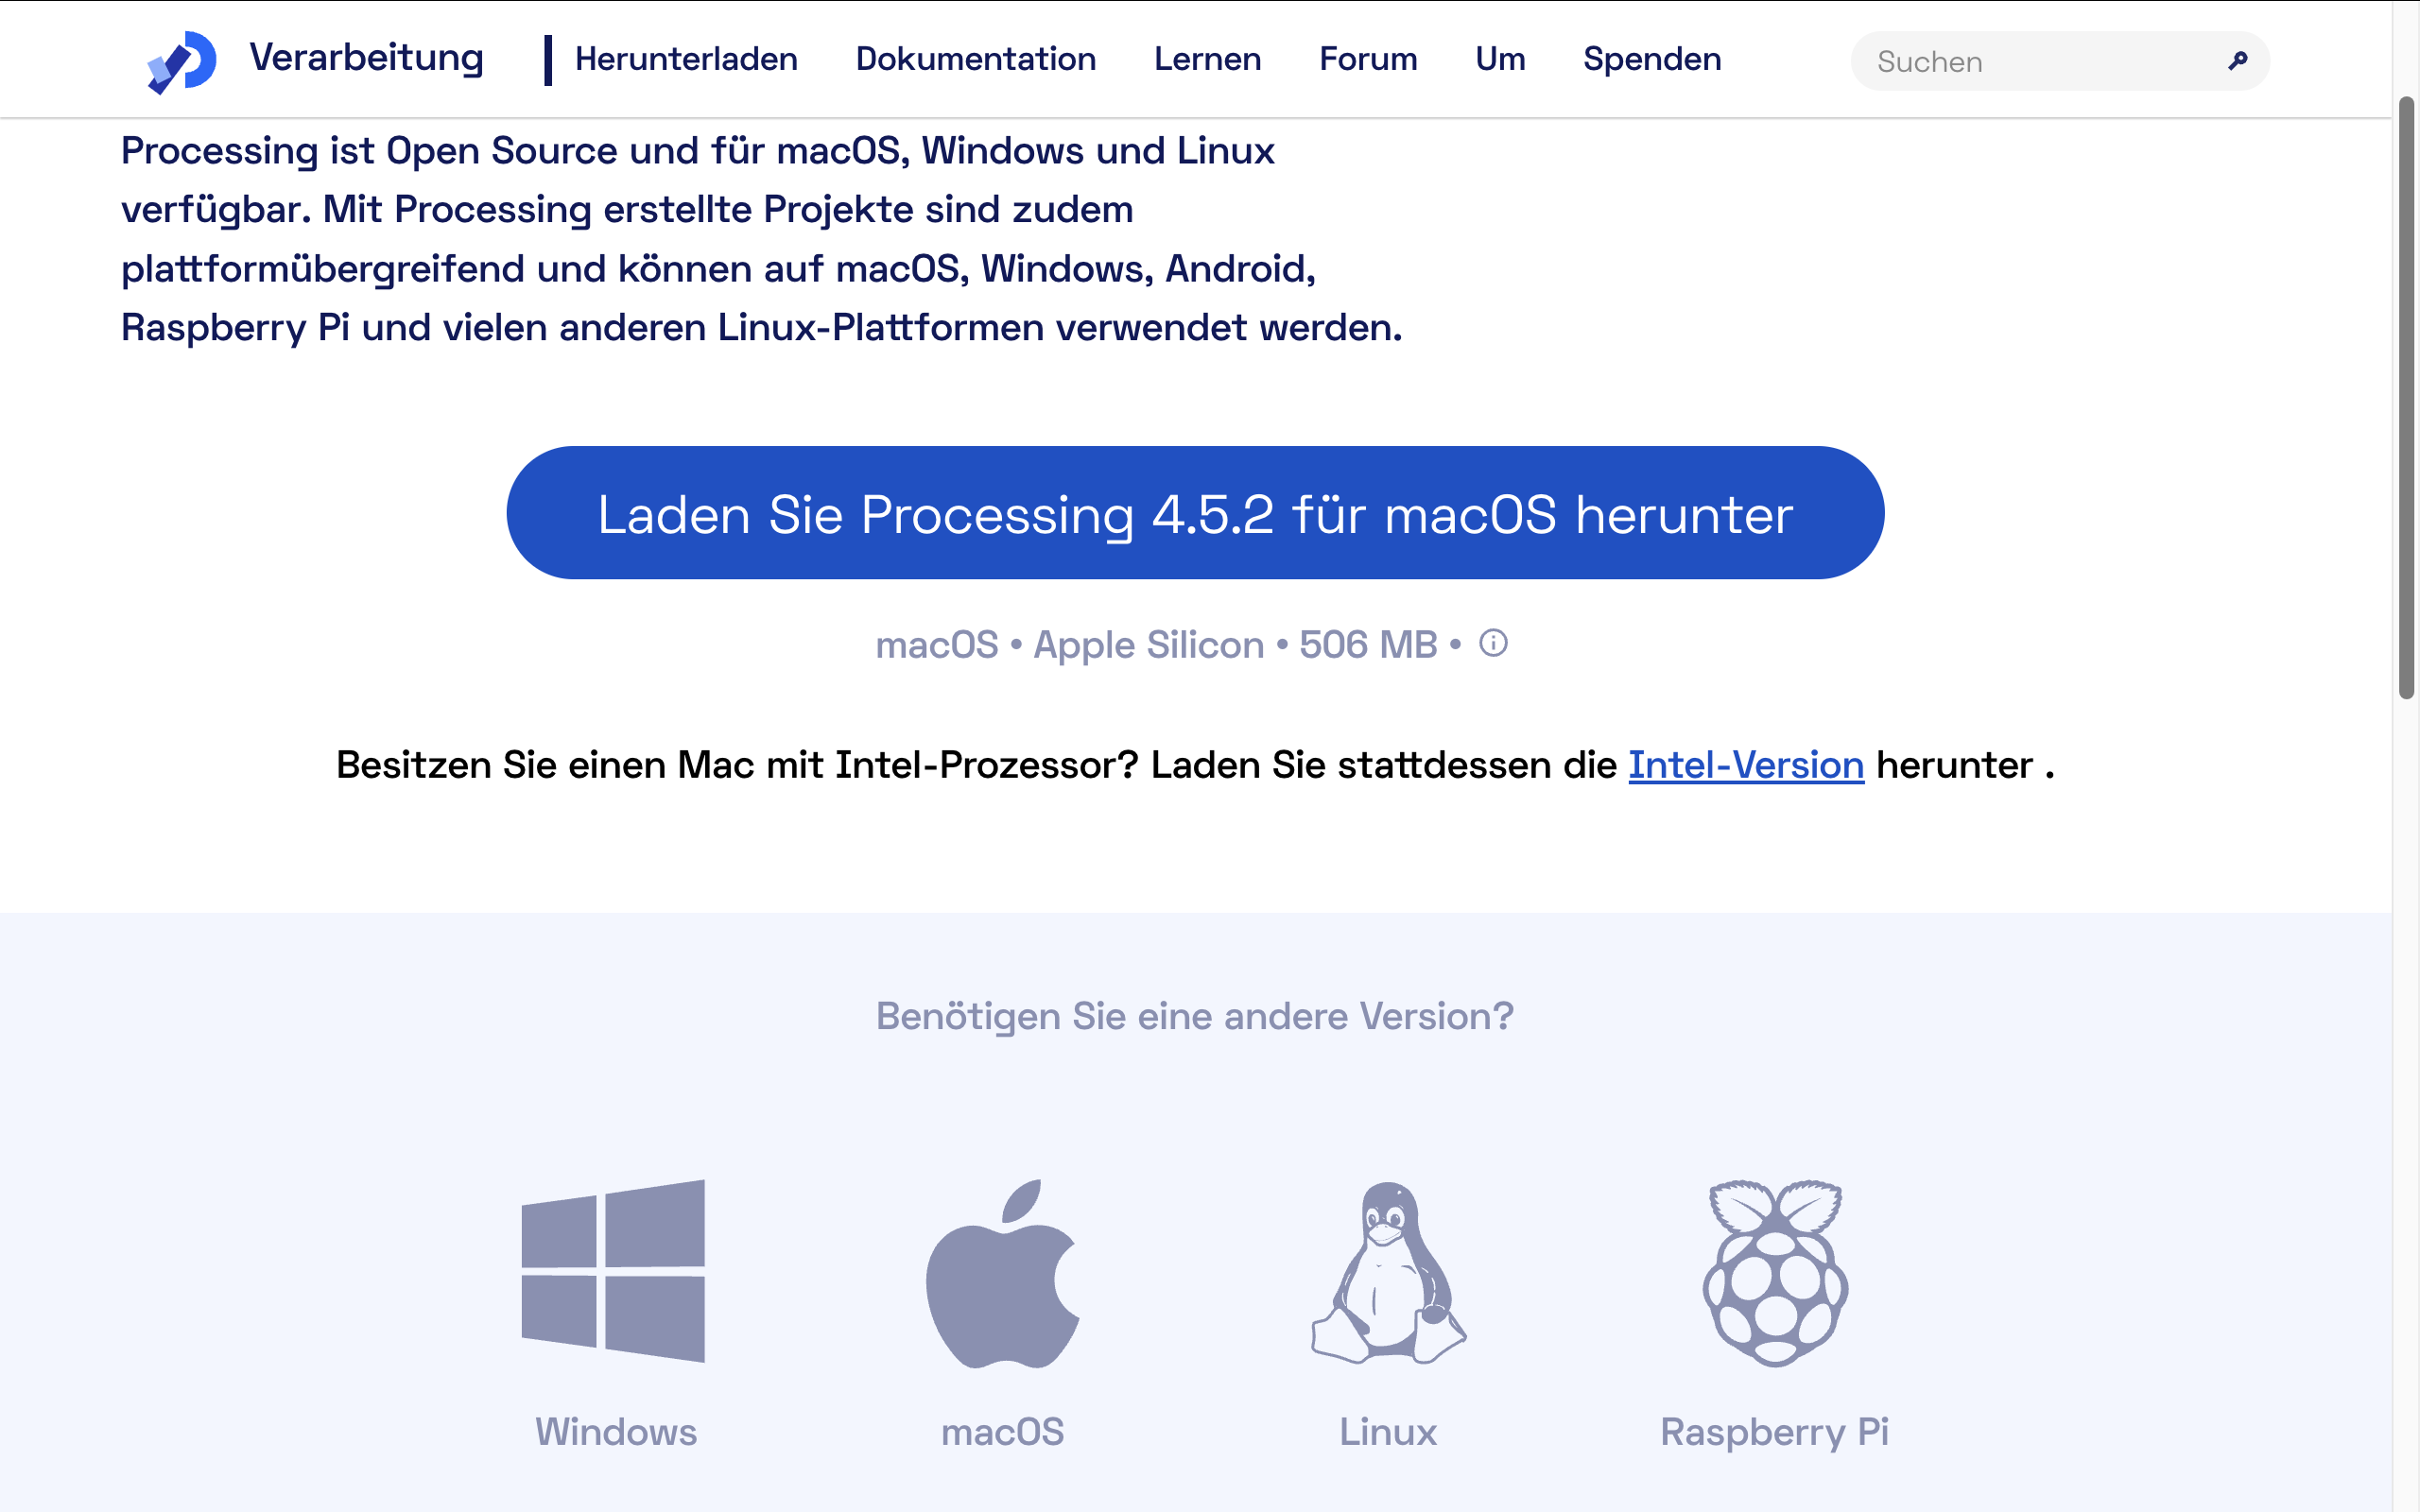
\includegraphics[width=\linewidth]{../Images/Processing/DownloadProcessing}
	\captionof{figure}{Processing Downloadverzeichnis}
	\label{fig:Download_Processing}
\end{center}

\subsection{Anforderungen Betriebssystem}
Die Systemanforderungen von Processing sind plattformübergreifend optimiert. Um eine stabile Render-Performance der Grafik-Pipelines (insbesondere bei der Nutzung von OpenGL- oder P3D-Renderern) zu gewährleisten, müssen die Hardwarekomponenten und das Betriebssystem die folgenden Mindestanforderungen erfüllen:
\begin{itemize}
	\item Windows: Windows 10 oder neuer, 64-Bit Intel- oder AMD-Prozessor
	\item Linux: 64-Bit (Kernel-Spezifikationen entsprechend der gängigen Distributionen wie Ubuntu)
	\item macOS: Intel-Architektur, Version 10.15 („Catalina“) oder neuer, 64-Bit
	\item macOS: Apple Silicon (M1/M2/M3), Version 11 („Big Sur“) oder neuer, native ARM-Unterstützung
\end{itemize}

\subsection{Installation auf Windows}
Die Einrichtung unter Windows erfordert keinen klassischen Windows-Installer, sondern wird als portable Anwendung bereitgestellt. Nach dem Download der Archivdatei \FILE{processing-4.3-windows-x64.zip} wird diese per Rechtsklick entpackt. Der resultierende Ordner kann in ein beliebiges Verzeichnis verschoben werden (z.,B. \FILE{C:/Programme/}). Die Entwicklungsumgebung wird anschlie\ss lich durch einen Doppelklick auf die ausführbare Datei \FILE{processing.exe} gestartet.

\subsection{Installation auf macOS}
Für macOS-Systeme liegt die Software als komprimiertes ZIP-Archiv vor. Nach dem automatischen Entpacken durch den Browser wird die Applikation \FILE{Processing.app} per Drag-and-Drop in den Systemordner \FILE{Programme} verschoben.

Beim ersten Start über ein Netzwerklaufwerk oder ein externes Speichermedium (wie einen USB-Stick) greifen die Sicherheitsmechanismen von macOS (Gatekeeper). Sollte das System den Start verweigern, kann die Quarantäne-Eigenschaft der Datei über das Terminal mittels des Befehls \SHELL{xattr -cr /Pfad/zu/Processing.app} aufgehoben werden. Nach dem erfolgreichen Bootvorgang präsentiert sich das Startfenster der IDE mit einem leeren Dokumenten-Template, wie in Abbildung~\ref{fig:Startfenster_Processing} illustriert.
\begin{center}\centering
	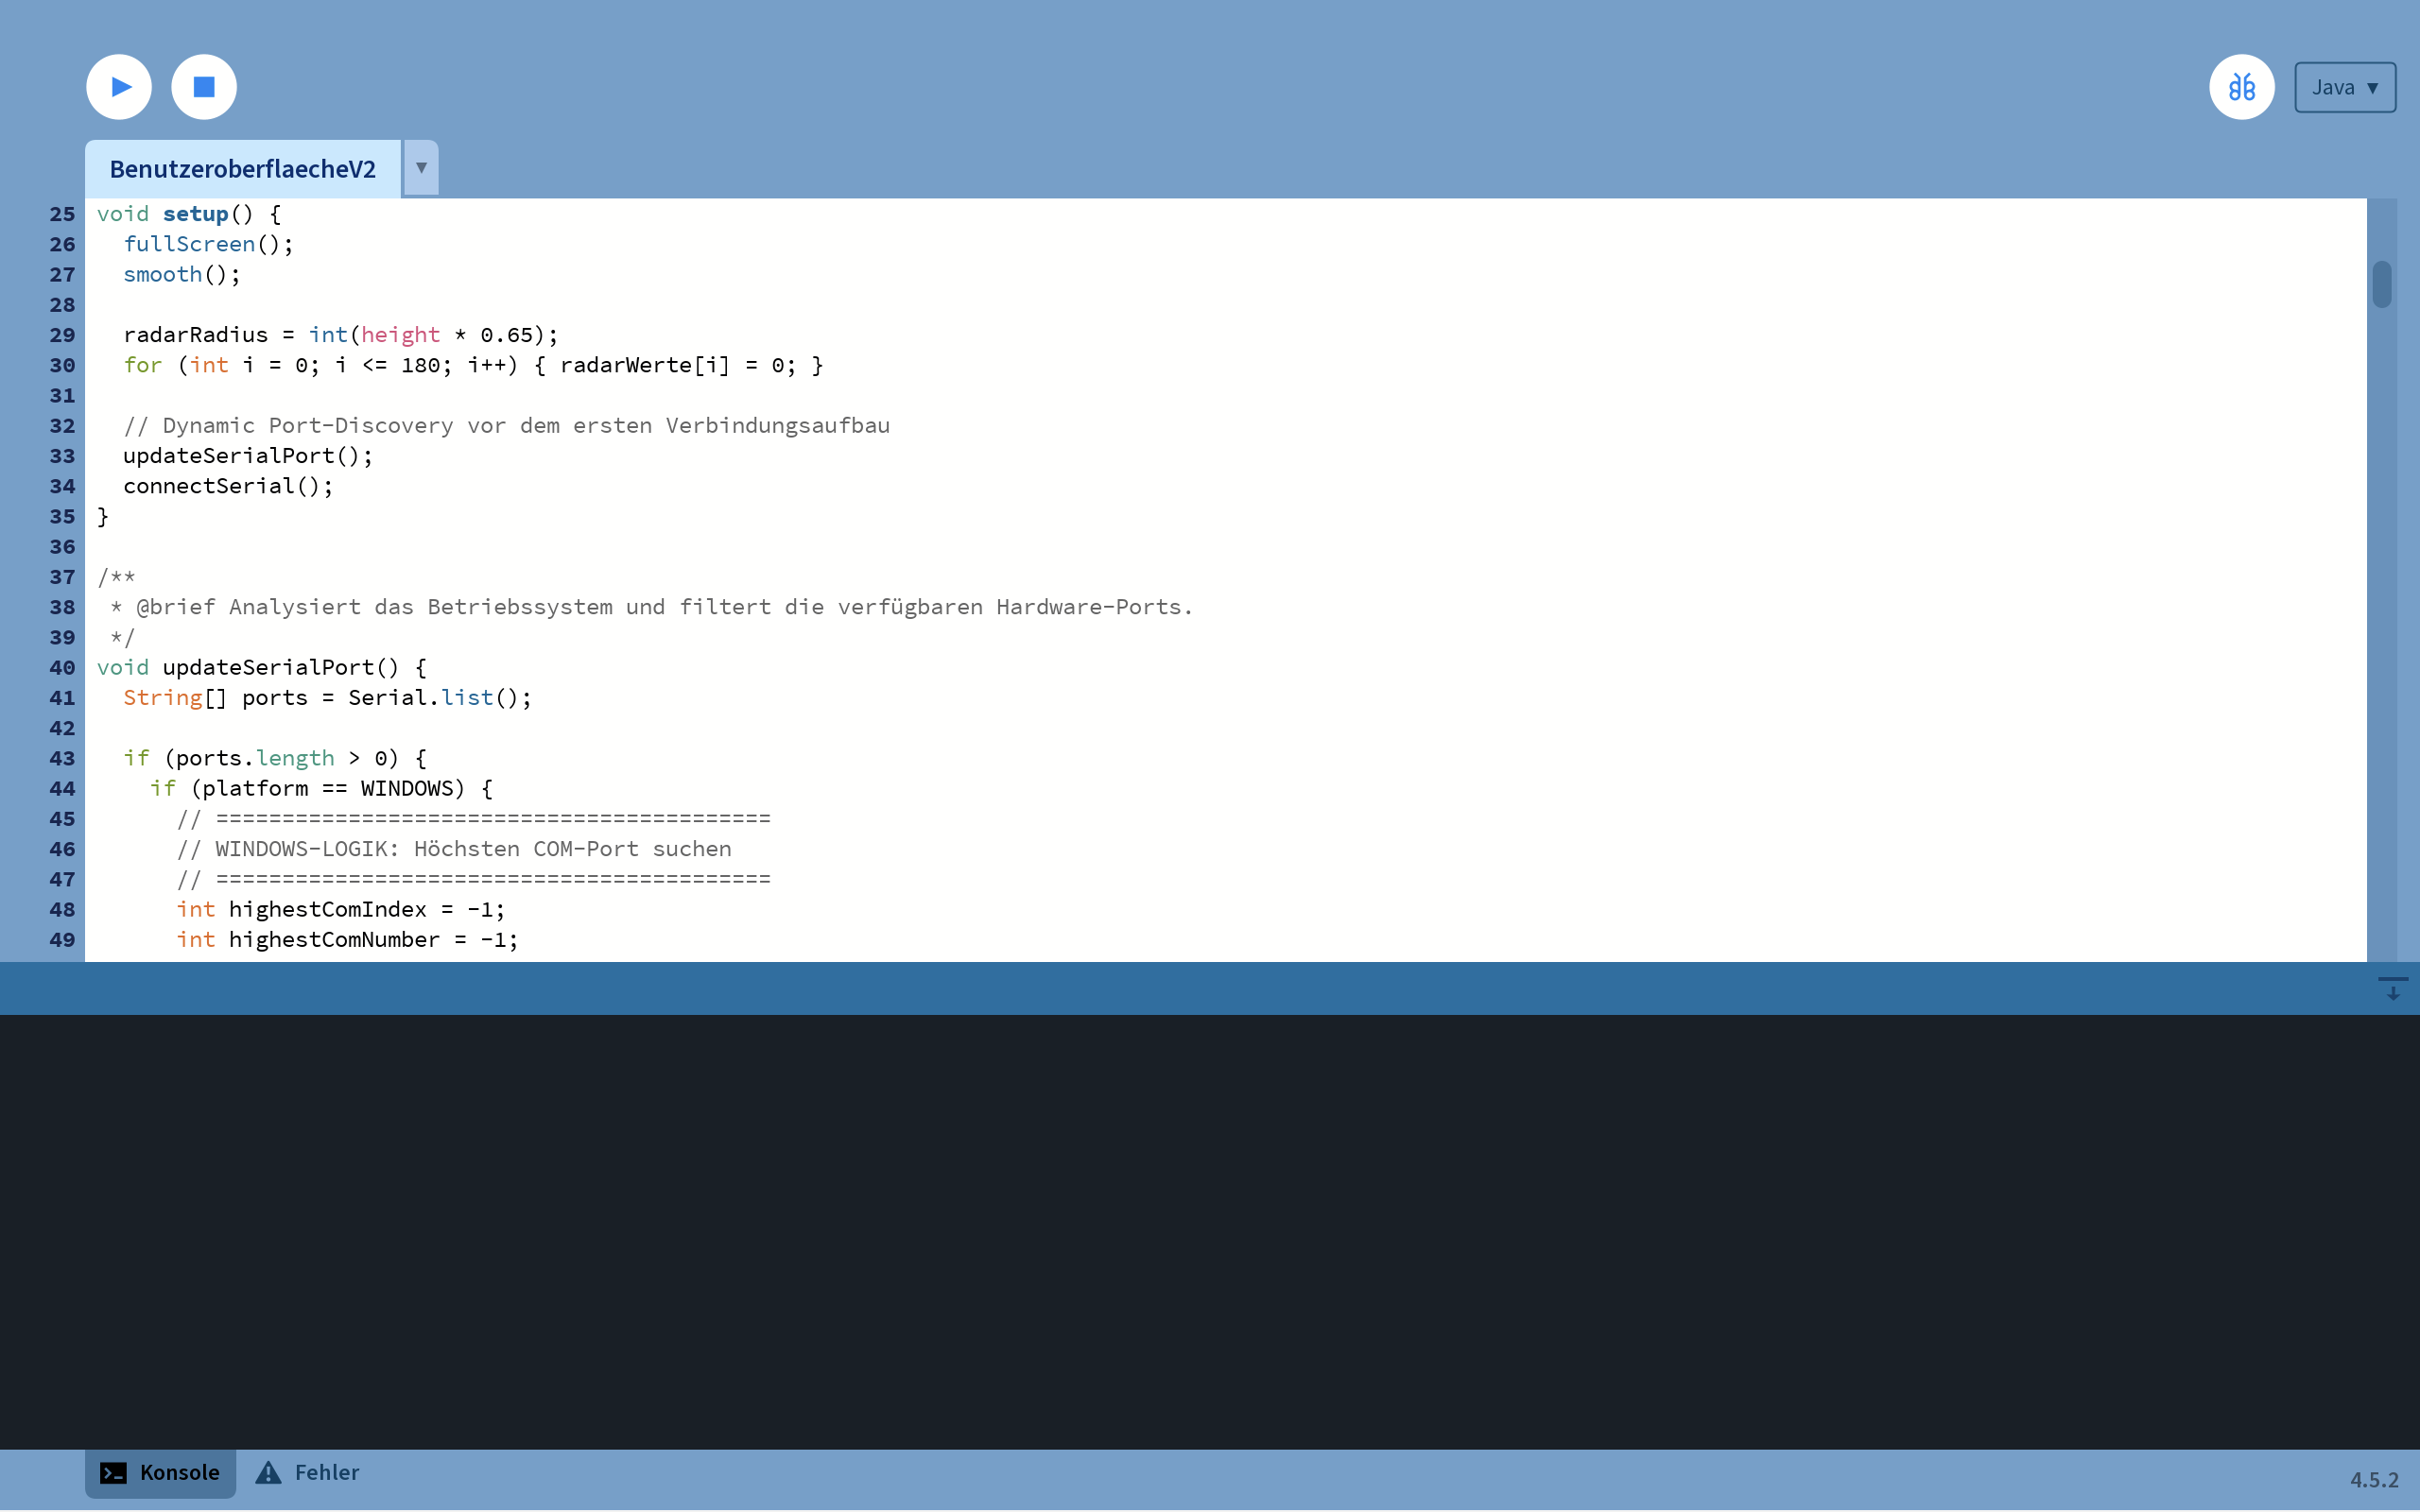
\includegraphics[width=\linewidth]{../Images/Processing/StartfensterProcessing.png}
	\captionof{figure}{Startfenster der Processing-IDE}\label{fig:Startfenster_Processing}
\end{center}

Das geöffnete Template zeigt die grundlegende Struktur. Obwohl einfache Skripte in Processing linear geschrieben werden können, basiert jede professionelle, interaktive Anwendung auf zwei tragenden Säulenstrukturen:
\\
Die Funktion \PYTHON{void setup()} wird beim Programmstart genau einmal aufgerufen. Hier werden grundlegende Systemeinstellungen vorgenommen, wie die Definition der Fenstergrö\ss e mittels \PYTHON{size()} oder \PYTHON{fullScreen()}, die Konfiguration des Antialiasing (\PYTHON{smooth()}) sowie das Öffnen von Kommunikationskanälen zu seriellen Ports.
\\
Die Funktion \PYTHON{void draw()} fungiert als kontinuierliche Zeichenschleife. Sie wird standardmä\ss ig exakt 60-mal pro Sekunde (60 Hz) aufgerufen. Innerhalb dieser Schleife wird das gesamte Radarbild in jedem Frame komplett neu gezeichnet, Sensor-Arrays ausgelesen und Hindernisse mathematisch berechnet. Durch das wiederholte Zeichnen entsteht für den Anwender die flie\ss ende Animation des rotierenden Radarstrahls.

\section{Übersicht der Eigenschaften und Contribution Manager}
\label{UebersichtUndEigenschaftenProcessing}
Über das Menü \menu{Skizze > Bibliothek hinzufügen > Bibliothek verwalten...} verfügt Processing über ein mächtiges Werkzeug zur modularen Code-Erweiterung: den Contribution Manager (Abbildung~\ref{fig:Contribution_Manager}).
\begin{center}
	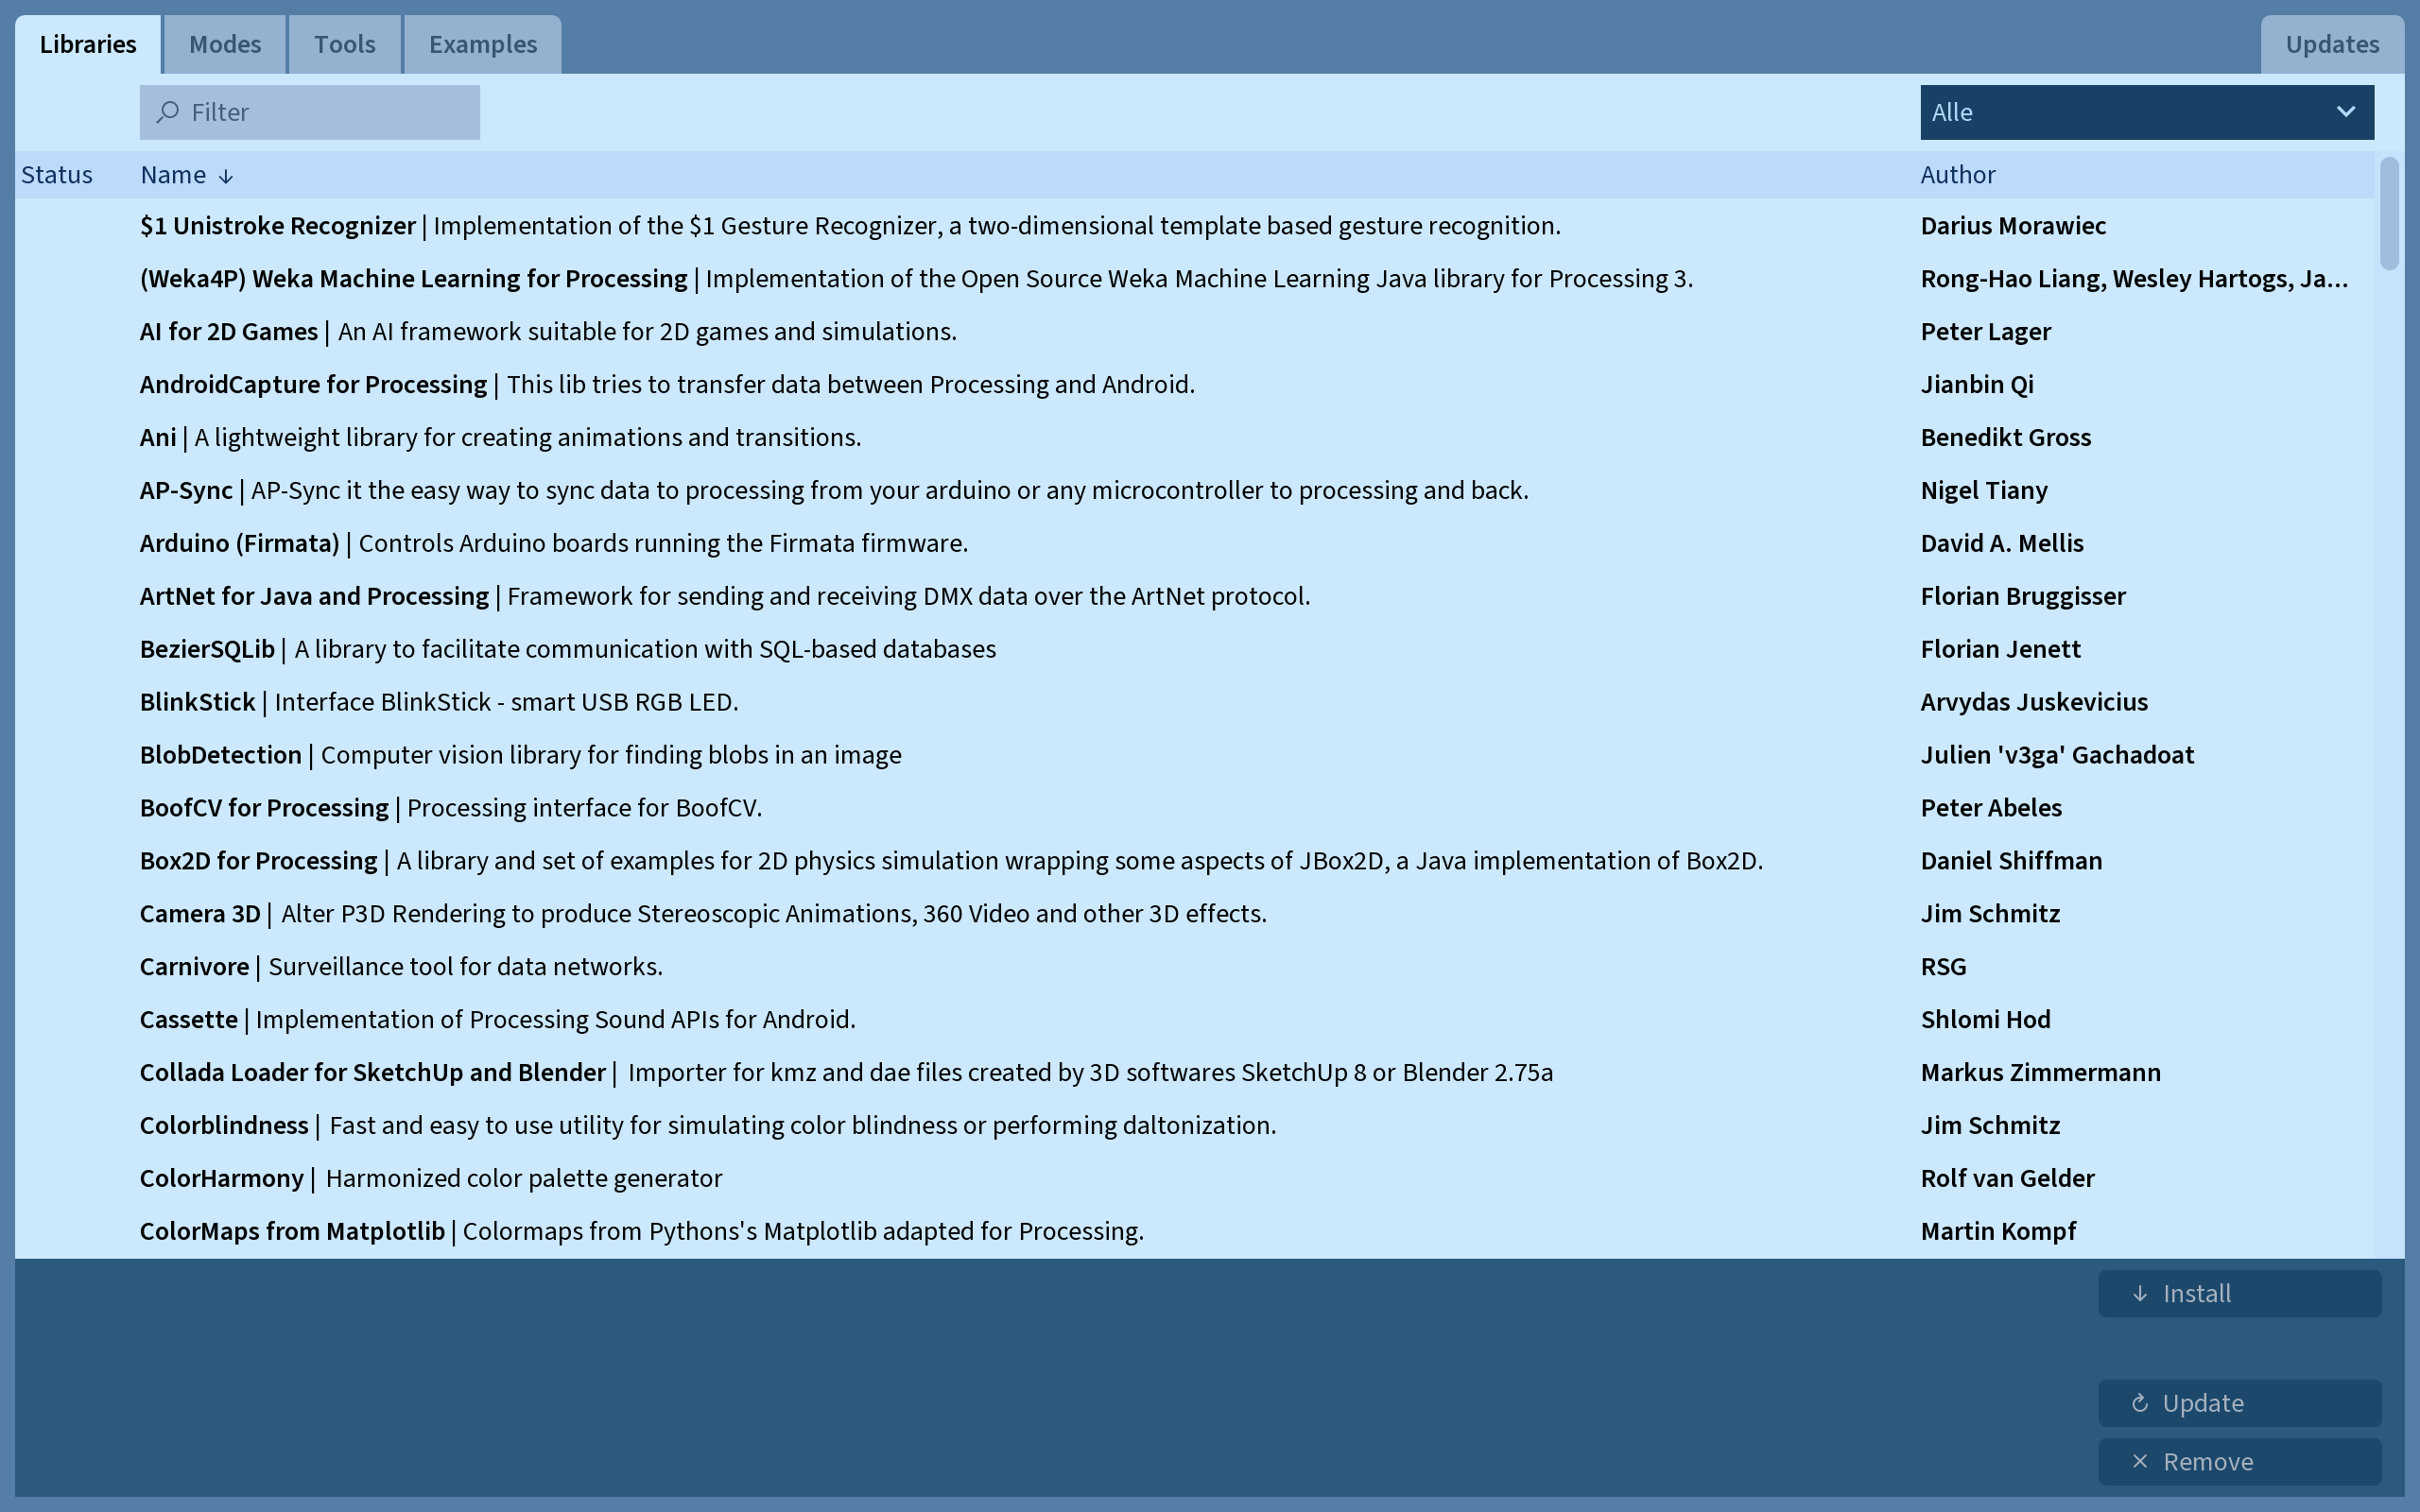
\includegraphics[width=\linewidth]{../Images/Processing/contributionManager.png}
	\captionof{figure}{Processing Contribution Manager}\label{fig:Contribution_Manager}
\end{center}
Der Contribution Manager gliedert sich in vier funktionale Bereiche:
\begin{itemize}
	\item \textbf{Libraries:} Ermöglicht das Durchsuchen und Installieren tausender Community-Bibliotheken zur Integration komplexer Hardwarekomponenten (z.,B. Videokameras, Sound-Engines oder Netzwerkschnittstellen).
	\item \textbf{Modes:} Erlaubt das Umschalten der Programmiersprache innerhalb der IDE (z.,B. von Java auf Python- oder JavaScript-Modus).
	\item \textbf{Tools:} Integriert nützliche Helferwerkzeuge direkt in den Editor, wie beispielsweise Farbwähler oder Font-Generatoren zur Erstellung benutzerdefinierter Pixelfonts.
	\item \textbf{Examples:} Lädt vollständige Beispiel-Projekte zu installierten Bibliotheken herunter.
\end{itemize}
\subsection{Die serielle Schnittstelle (Serial-Bibliothek)}
Für Hardware-Projekte, bei denen Messdaten von einem externen Mikrocontroller ausgewertet werden sollen, ist die Bibliothek \PYTHON{processing.serial.*} von essenzieller Bedeutung. Sie ist standardmä\ss ig im Kern von Processing enthalten, muss jedoch zu Beginn eines jeden Visualisierungs-Sketches explizit importiert werden:
\medskip
\PYTHON{import processing.serial.*;}
\medskip
Diese Bibliothek stellt das \PYTHON{Serial}-Objekt bereit, welches Interrupt-gesteuert im Hintergrund den Hardware-Puffer des gewählten COM- oder USB-Ports überwacht. Mittels Funktionen wie \PYTHON{myPort.readStringUntil n} können Datenpakete des Arduinos verlustfrei abgefangen, segmentiert und unmittelbar zur grafischen Darstellung an die \PYTHON{draw()}-Schleife übergeben werden.